%%%%%%%%%%%%%%%%%%%%%%%%%%%%%%%%%%%%%%%%%%%%%%%%%%%%%%%%%%%%%%%%%%%%%%%%%%%%%%%%
% Лабораторная работа 5 : Определение микротвердости.
% Выполнили             : Баталов Семен, Хайретдинова Диана, 2021.
%%%%%%%%%%%%%%%%%%%%%%%%%%%%%%%%%%%%%%%%%%%%%%%%%%%%%%%%%%%%%%%%%%%%%%%%%%%%%%%%

\documentclass[12pt, a4paper]{article}
\usepackage[left=2cm, right=2cm, top=2.5cm, bottom=2.5cm, nohead]{geometry}
\usepackage{graphicx}
\usepackage[utf8]{inputenc}
\usepackage[english, russian]{babel}
\usepackage{indentfirst}
\usepackage{amsmath}
\usepackage{longtable}
\usepackage{multirow}
\usepackage{array}
\usepackage{rotating}
\usepackage{subcaption}
\graphicspath{{./Figures/}}

\begin{document}
    
    \newcolumntype{M}[1]{>{\centering\arraybackslash}m{#1}}
    \renewcommand{\arraystretch}{1.3}
    
    \begin{center}
        \large{Санкт-Петербургский Государственный Университет} \\
        \large{Saint-Petersburg State University}\\
        \hfill \break
        \hfill \break
        \hfill \break
        \hfill \break
        \hfill \break
        \hfill \break
        \large{ЛАБОРАТОРИЯ ПРОЧНОСТИ МАТЕРИАЛОВ} \\
        \hfill \break
        \hfill \break
        \hfill \break
        \large{\textbf{ОТЧЕТ}} \\
        \large{\textbf{По лабораторной работе 5}} \\
        \large{<<Определение микротвердости>>} \\
        \hfill \break
        \hfill \break
        \hfill \break
        \large{По дисциплине} \\
        \large{<<Лабораторный практикум, лабораторная работа>>} \\
    \end{center}
    
    \hfill \break
    \hfill \break
    \hfill \break
    \hfill \break
    \hfill \break
    \hfill \break
    
    \begin{flushright} 
        \large{Выполнили:} \\
        \hfill \break
        \large{Баталов С. А.} \\
        \large{Хайретдинова Д. Д.} \\
    \end{flushright}
    
    \hfill \break
    \hfill \break
    \hfill \break
    \hfill \break
    \hfill \break
    
    \begin{center} 
        \large{Санкт-Петербург} \\
        \large{2021} \\
    \end{center}
    
    \thispagestyle{empty}
    \newpage
    \sloppy
    
    \section{Цель работы}
    
    Понятие <<твердость>> широко распространено и часто применяется в повседневной жизни. Различают твердые и мягкие вещества без определения или численного выражения твердости. В технике наиболее часто понятие твердость определяют как сопротивление, оказываемое телом при внедрении в него другого, более твердого тела. Герц попытался дать понятию <<твердость>> физически более точный смысл и определил ее как предельную нагрузку, которая еще не вызывает остаточной деформации материала. Однако точное определение подобных величин твердости связано с большими трудностями, и они не смогли утвердиться в технике. В настоящее время под «твердостью» понимают свойство поверхностного слоя материала оказывать сопротивление упругой и пластической деформации или разрушению при местных контактных воздействиях со стороны другого, более твердого и не получающего остаточной деформации тела (индентора) определенной формы и размера.
    
    В данной работе будет проведено экспериментальное определение микротвердости (твёрдость отдельных участков микроструктуры материала) образца. Исследование будет проведено на специальной измерительной машине, принцип работы которой заключается во внедрении индентора (это изготовленный из алмаза, твердого сплава или закаленной стали наконечник прибора, используемого для измерения твердости) в образец и анализе полученных пластических деформаций.
    
    Основными целями работы являются: измерение микротвердости алюминиевого и стального образцов, исследование влияния нагрузки на величину микротвердости стали, исследование влияния длительности индентирования на величину микротвердости алюминия, проведение статистической обработки результатов экспериментов.
    
    \newpage
    
    \section{Экспериментальная установка}
    
    Для измерения микротвердости используют различные приборы (ПМТ-3, Buehler). В лаборатории прочности материалов математико-механического факультета СПбГУ для определения микротвердости используют прибор  Buehler Micromet 5103 фотография, которого представлен на рис.~\ref{im1}. Прибор состоит из предметного столика I с держателем образца II, оптической системы III, индентора и нагружающей системы IV, фотоаппарата V, блока управления VI, компьютера VII.
    
    \begin{figure}[h]
        \centering
        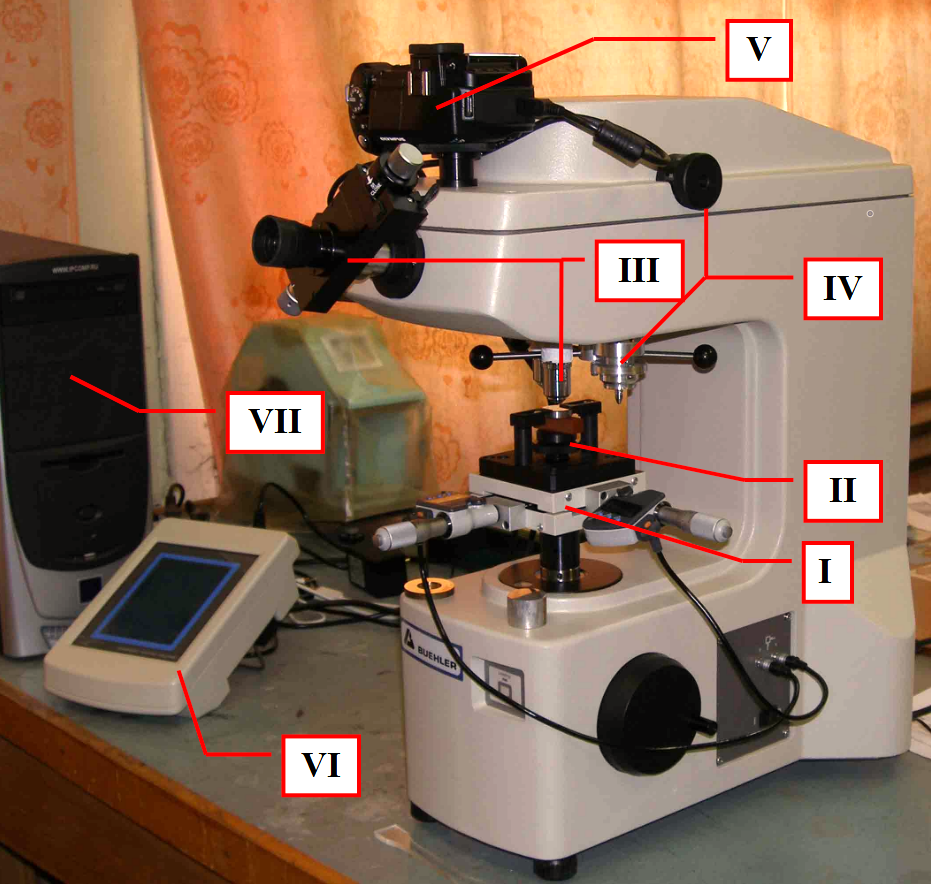
\includegraphics[width = 14cm]{image_1.png}
        \caption{Микротвердомер Buehler Micromet 5103.}
        \label{im1}
    \end{figure}
    
    С помощью системы видеозахвата фотоаппарат соединен с компьютером, что позволяет передавать фотографии отпечатков на компьютер с целью дальнейшей обработки информации. Кроме этого специальное программное обеспечение позволяет управлять параметрами съемки поверхности образца непосредственно с компьютера. Для управления работой фотоаппарата используется программа <<Olympus Studio>>, для обработки экспериментальных  результатов (определение диагоналей отпечатка индентора, вычисления числа микротвердости, построения статистического распределения данных эксперимента) используется <<ImageExpert MicroHardness>>.
    
    \newpage
    
    \section{Теоретические исследования}
    
    \subsection{Расчет микротвердости}
    
    При определении микротвредости (в отличие от макротвердости) используют малые нагрузки (до 2~Н). В этом случае удается получить характеристики твердости в специфических областях. Например, можно измерить твердость отдельных кристаллитов, включений или границ зерен. 
    
    Микротвердость может быть измерена различными методами, которые отличаются друг от друга формой индентора и способом расчета микротвердости. В большинстве случаев в качестве индентора, как и в случае определения твердости по Виккерсу, используют правильную четырехгранную алмазную пирамиду с углом при вершине $136^\circ$. Тогда число микротвердости определяется как отношение нагрузки $P$ (в [г]) к площади боковой поверхности полученного пирамидального отпечатка $S$ (в [мкм]):
    \begin{equation}
        H = \frac{P}{S},
        \label{eq1}
    \end{equation}
    площадь бокового отпечатка можно найти по формуле:
    \begin{equation}
        S = \frac{d^2}{2} \cdot \frac{1}{sin \, 68^\circ},
        \label{eq2}
    \end{equation}
    где $d$~--~диагональ отпечатка в мкм. Тогда твердость будет определяться по формуле:
    \begin{equation}
        H = \frac{2Psin \, 68^\circ}{d^2} = \frac{1.854 P}{d^2}, \quad HV = 1000 \cdot H.
        \label{eq3}
    \end{equation}
    
    Число микротвердости записывают без размерности с указанием величины нагрузки в [гс], например,  $H_5-300$, $H_{20}-250$.
    
    \subsection{Статистическая обработка результатов}
    
    Совокупность значений механических свойств обыч­но хорошо подчиняется нормальному закону распределения. Поэтому среднее значение $x$ какого-либо свойства по результатам $n$ измерений в большинстве случаев расчитывают как среднее арифметическое:
    \begin{equation}
        \overline{x} = \frac{1}{n} \sum_{i=1}^{n} x_{i}.
        \label{eq4}
    \end{equation}
    
    Для оценки ошибки отдельных измерений определяют их отклонение от среднего в виде дисперсии:
    \begin{equation}
        s^{2} = \frac{1}{n-1} \sum_{i=1}^{n} (x_{i} - \overline{x})^{2},
        \label{eq5}
    \end{equation}
    или среднего квадратичного отклонения (стандартного отклонения) отдельного измерения:
    \begin{equation}
        s = \sqrt{\frac{1}{n-1} \sum_{i=1}^{n} (x_{i} - \overline{x})^{2}}.
        \label{eq6}
    \end{equation}
    
    Важной характеристикой точности изменений является также относительная величина среднего квадратичного отклонения~--~коэффициент вариации:
    \begin{equation}
        W = \frac{s}{\overline{x}} \cdot 100\%.
        \label{eq7}
    \end{equation}
    
    Наиболее точную оценку величины ошибок дает доверительный интервал в сочетании с доверительной вероятностью. Обозначим погрешность измерения истинной величины измеряемого свойства через $\Delta x$. Предположим теперь, что вероятность отличия $\overline{x}$ от $x$ на величину, не большую чем $\Delta x$, равна $\alpha$:
    \begin{equation}
        P(-\Delta x < x - \overline{x} < \Delta x) = \alpha,
        \label{eq8}
    \end{equation}
    вероятность $\alpha$ называется доверительной вероятностью, а интервал значений от $\overline{x} - \Delta x$ до $\overline{x} + \Delta x$ называется доверительным интервалом.
    
    Величина доверительного интервала определяется средним значением $\overline{x}$, средним квадратичным отклонением $s$ и критерием Стьюдента $t = t(\alpha, \, n)$:
    \begin{equation}
        x \in \bigg (\overline{x} - \frac{s}{\sqrt{n}} \cdot t, \, \overline{x} + \frac{s}{\sqrt{n}} \cdot t \bigg ).
        \label{eq9}
    \end{equation}
    
    Погрешность косвенных измерений для функции $f(x_{1}, \, \ldots, \, x_{m})$ расчитываем по стандартной формуле:
    \begin{equation}
        \Delta f = \sqrt{\Bigg( \frac{\partial f(\overline{x_{1}})}{\partial x_{1}} \cdot \Delta x_{1}\Bigg )^{2} + \ldots + \Bigg( \frac{\partial f(\overline{x_{1}})}{\partial x_{m}} \cdot \Delta x_{m}\Bigg )^{2}}.
        \label{eq10}
    \end{equation}
    
    \newpage
    
    \section{Эксперимент}
    
    Сначала определяем микротвердость стали и алюминия при постоянном усилии $P$ и продолжительности $t$ воздействия индентора. Результаты опытов приведены ниже.
    
    \begin{table}[h]
        \centering
        \begin{tabular}{|M{1cm}|M{2.5cm}|M{1cm}|M{1cm}|M{1.5cm}|M{1.5cm}|M{1.5cm}|M{1.5cm}|}
            \hline
            \multirow{2}{*}{№} & \multirow{2}{*}{Материал} & $P$ & $t$ & $d_{1}$ & $d_{2}$ & $d_{\text{ср}}$ & $HV$ \\
            \cline{3-8}
            & & г & с & \multicolumn{3}{c|}{мкм} & -- \\
            \hline
            1 & \multirow{10}{*}{Сталь} & \multirow{10}{*}{200} & \multirow{10}{*}{10} & 50.5 & 50.3 & 50.4 & 146.0 \\
            2 & & & & 49.2 & 46.2 & 47.7 & 163.3 \\
            3 & & & & 48.6 & 48.2 & 48.4 & 158.2 \\
            4 & & & & 43.2 & 42.2 & 42.7 & 203.8 \\
            5 & & & & 49.8 & 46.7 & 48.3 & 159.2 \\
            6 & & & & 49.3 & 49.0 & 49.1 & 153.7 \\
            7 & & & & 46.2 & 45.6 & 45.6 & 176.2 \\
            8 & & & & 48.3 & 47.2 & 47.8 & 162.6 \\
            9 & & & & 45.3 & 44.8 & 45.0 & 182.8 \\
            10 & & & & 47.9 & 47.1 & 47.5 & 164.4 \\
            \hline
            1 & \multirow{10}{*}{Алюминий} & \multirow{10}{*}{200} & \multirow{10}{*}{10} & 52.1 & 51.1 & 51.6 & 139.2 \\
            2 & & & & 53.2 & 51.5 & 52.4 & 135.1 \\
            3 & & & & 53.6 & 52.0 & 52.8 & 133.2 \\
            4 & & & & 53.1 & 50.8 & 52.0 & 137.4 \\
            5 & & & & 54.4 & 53.3 & 53.8 & 128.0 \\
            6 & & & & 54.0 & 53.3 & 53.6 & 128.9 \\
            7 & & & & 51.6 & 51.1 & 51.4 & 134.5 \\
            8 & & & & 51.6 & 51.1 & 51.4 & 140.5 \\
            9 & & & & 50.7 & 50.1 & 50.4 & 145.9 \\
            10 & & & & 54.3 & 54.0 & 54.2 & 126.4 \\
            \hline
        \end{tabular}
        \caption{\centering Исследование микротвердости стального и алюминиевого образцов.}
        \label{tb1}
    \end{table}
    
    Данные твердости в таблице получены при автоматическом расчете программного модуля <<ImageExpert MicroHardness>>. В таблице~\ref{tb2} представлены результаты измерения микротвердости стали при различной нагрузке $P$ и микротвердости алюминия при различном времени удержания $t$.
    
    Перейдем к статистической оценке результатов. Рассчитаем по известным формулам: среднее значение, дисперсию, среднеквадратичное отклонение, коэффициент вариации, погрешность как прямых, так и косвенных измерений. Все полученные значения запишем в таблицу~\ref{tb3}. Для вычисления и построения графиков используем пакет Matlab, с программным кодом можно ознакомиться отдельно.
    
    Важно отметить, что в таблице~\ref{tb3} сначала расчитываются значения $\overline{d_{1}}$ и $\overline{d_{2}}$, только после этого производится расчет остальных величин.
    
    \newpage
    
    \begin{table}[h]
        \centering
        \begin{tabular}{|M{1cm}|M{2.5cm}|M{1cm}|M{1cm}|M{1.5cm}|M{1.5cm}|M{1.5cm}|M{1.5cm}|}
            \hline
            \multirow{2}{*}{№} & \multirow{2}{*}{Материал} & $P$ & $t$ & $d_{1}$ & $d_{2}$ & $d_{\text{ср}}$ & $HV$ \\
            \cline{3-8}
            & & г & с & \multicolumn{3}{c|}{мкм} & -- \\
            \hline
            1 & \multirow{8}{*}{Сталь} & 10 & \multirow{8}{*}{10} & 8.6  & 8.5 & 8.6 & 252.8 \\
            2 & & 25 & & 20.1 & 19.0 & 19.5 & 121.5 \\
            3 & & 50 & & 25.9 & 22.8 & 24.4  & 156.1 \\
            4 & & 100 & & 33.1 & 32.1 & 32.6 & 174.6 \\
            5 & & 200 & & 48.3 & 47.2 & 47.8 & 162.6 \\
            6 & & 300 & & 57.3 & 56.9 & 57.1 & 170.4 \\
            7 & & 500 & & 76.1 & 75.8 & 75.9 & 160.9 \\
            8 & & 1000 & & 108.4 & 107.3 & 107.9 & 159.4 \\
            \hline
            1 & \multirow{5}{*}{Алюминий} & \multirow{5}{*}{200} & 5 & 51.0 & 50.0 & 50.5 & 145.4 \\
            2 & & & 10 & 53.1 & 50.8 & 52.0 & 137.4 \\
            3 & & & 20 & 52.8 & 51.9 & 52.4 & 135.3 \\
            4 & & & 40 & 52.3 & 51.8 & 52.8 & 136.9 \\
            5 & & & 60 & 52.5 & 51.5 & 52.0 &  137.1 \\
            \hline
        \end{tabular}
        \caption{\centering Исследование микротвердости стального и алюминиевого образцов в зависимости от прикладываемой нагрузки и продолжительности удержания.}
        \label{tb2}
    \end{table}
    
    \begin{table}[h]
        \centering
        \begin{tabular}{|M{3cm}|M{1cm}|M{1cm}|M{1cm}|M{1cm}|M{1cm}|M{1cm}|M{1cm}|M{1cm}|}
            \hline
            Материал & \multicolumn{4}{c|}{Сталь} & \multicolumn{4}{c|}{Алюминий} \\
            \hline
            Величина & $\overline{d_{1}}$ & $\overline{d_{2}}$ & $d_{\text{ср}}$ & $HV$ & $\overline{d_{1}}$ & $\overline{d_{2}}$ & $d_{\text{ср}}$ & $HV$ \\
            \hline
            Размерность & \multicolumn{3}{c|}{мкм} & -- & \multicolumn{3}{c|}{мкм} & -- \\
            \hline
            $\overline{x}$ & 48 & 47 & 47 & 166 & 53 & 52 & 52 & 135 \\
            $\Delta x$ & 1 & 1 & 1 & 6 & 1 & 1 & 1 & 3 \\
            \hline
            $s^{2}$ & 5.2 & 5.1 & -- & -- & 1.7 & 1.6 & -- & -- \\
            $s$ & 2.3 & 2.3 & -- & -- & 1.3 & 1.3 & -- & -- \\
            $W$,~\% & 5 & 5 & -- & -- & 2 & 2 & -- & -- \\
            $\varepsilon$,~\% & 2.1 & 2.1 & 2.1 & 3.6 & 1.9 & 1.9 & 1.9 & 2.2 \\
            \hline
        \end{tabular}
        \caption{\centering Статистическая оценка результатов.}
        \label{tb3}
    \end{table}
    
    Далее перейдем к построению графиков зависимости микротвердости от действующей нагрузки и зависимости микротвердости от времени индентирования. На рис.~\ref{fig1} изображена зависимость микротвердости стали от величины приложенной нагрузки, а также изображена зависимость микротвердости алюминия от длительности индентирования.
    
    \newpage
    
    \begin{figure}[h!]
        \centering
        \begin{subfigure}{\textwidth}
            \centering
            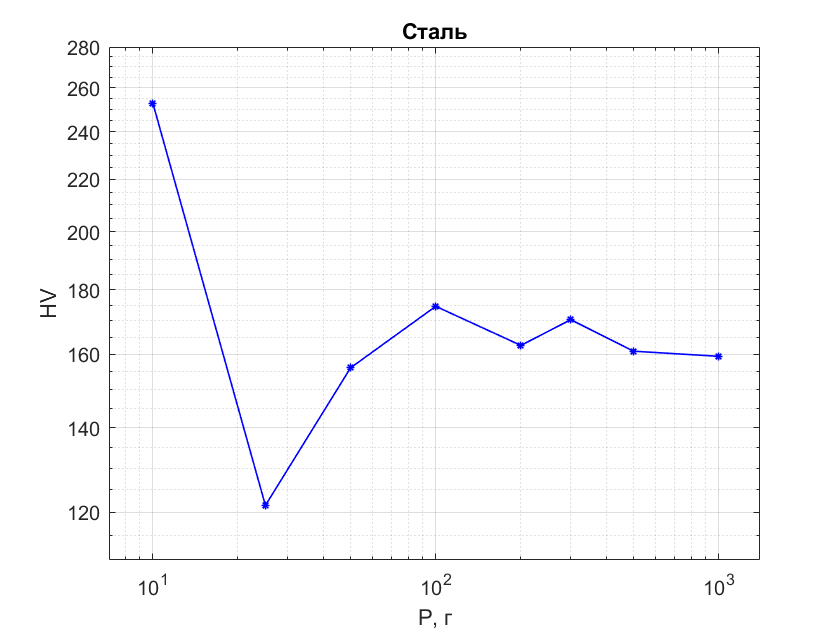
\includegraphics[width = 14cm]{figure_1.png}
        \end{subfigure}
        \begin{subfigure}{\textwidth}
            \centering
            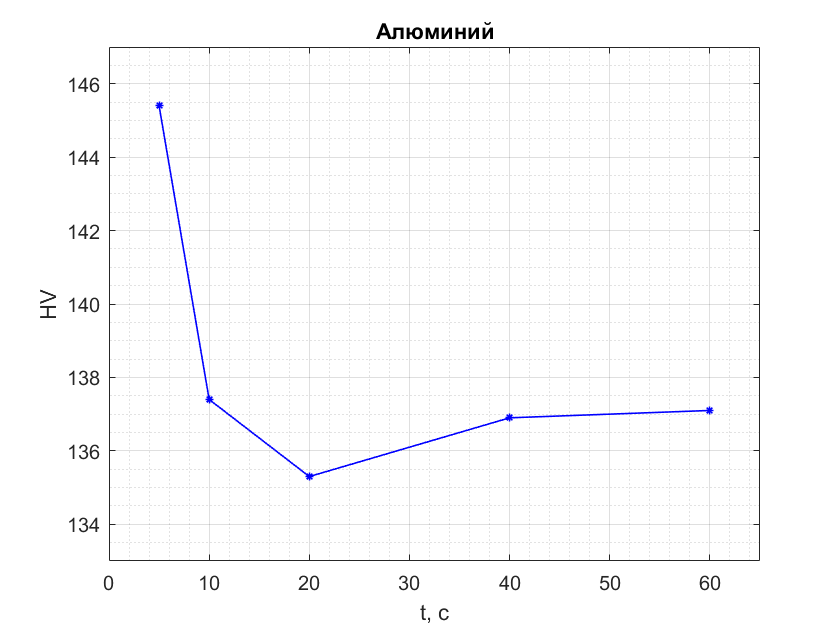
\includegraphics[width = 14cm]{figure_2.png}
        \end{subfigure}
        \caption{\centering Графики зависимости микротвердости от действующей нагрузки и зависимости микротвердости от времени индентирования.}
        \label{fig1}
    \end{figure}
    
    \newpage
    
    \section{Выводы}
    
    В данной работе было успешно проведено экспериментальное определение микротвердости образцов из алюминия и стали. Исследование было проведено на специальной измерительной машине, принцип работы которой заключается во внедрении индентора в образец и анализе полученных пластических деформаций. В процессе работы были изучены методы определения макротвердости и микротвердости, основанные на внедрении индентора в образец.
    
    Основные цели работы (измерение микротвердости алюминиевого и стального образцов, исследование влияния нагрузки на величину микротвердости стали, исследование влияния длительности индентирования на величину микротвердости алюминия, проведение статистической обработки результатов экспериментов) были выполнены.
    
\end{document}